\section{Aufgabenstellung}
\begin{enumerate}
\item Bestimmung der Gitterkonstanten aus dem räumlichen Abstand der 1. Beugungsordnungen von der 0. Ordnung.\\
\item Vermessung von 5 unterschiedlichen Amplitudengittern: Bestimmung ihrer Gitterkonstanten und ihres Auflösungsvermögens bei voller Ausleuchtung.\\
\item Bestimmung der Aperturfunktion für Gitter Nr. 1 aus den gemessenen Intensitäten der unterschiedlichen Beugungsordnungen und Auftragen einer Periode der so bestimmten Funktion.\\
\item Bestimmung des Verhältnisses von Spaltbreite zu Gitterkonstante mithilfe der Aperturfunktion.\\
\item
\begin{enumerate}
\item Vermessung der Intensitätsverteilung der entstehenden Beugungsfigur eines Ultraschall-Phasengitters in Abhängigkeit von der am Quarz anliegenden Spannung.\\
\item Vergleich der erhaltenen Ergebnisse mit der Raman-Nath-Theorie.
\item Bestimmung der Wellenlänge von Schall in Isooktan durch Messung unterschiedlicher Beugungsordnungen. Vergleich mit dem theoretischen Wert.
\end{enumerate}
\end{enumerate}
\clearpage
\section{Theoretische Grundlagen}
\subsection{Schematischer Aufbau}
\begin{center}
\begin{figure}[htbp]
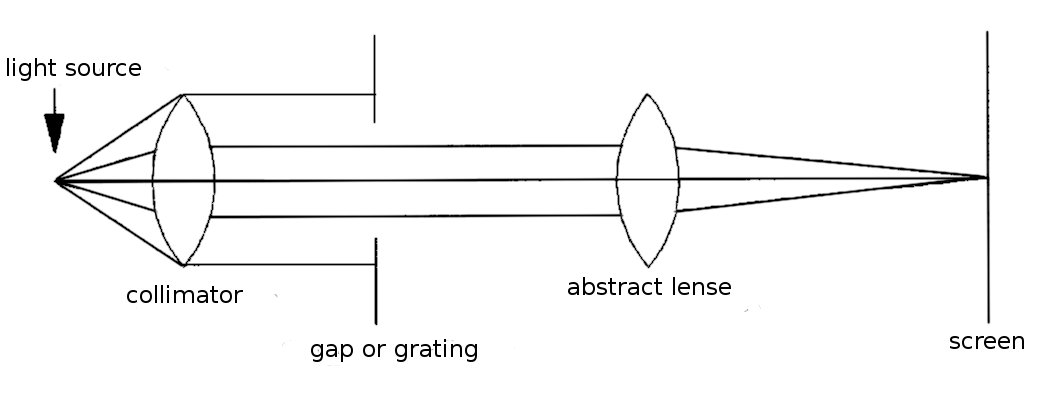
\includegraphics[scale=0.6]{Bilder/fraunhofer}
\caption{Fraunhofersche Anordnung, Quelle: [ver]}
\end{figure}
\end{center}
Beim Einfall einer Lichtwelle auf einen hinreichend engen Spalt (bzw. ein anderes geeignetes Hindernis) kann man auf einem Schirm hinter dem Spalt ein Beugungsbild beobachten. Im Wesentlichen liefert das Huygenssche Prinzip eine gute Vorstellung: Jeder Punkt des Spaltes lässt sich als Erregerzentrum einer Elementarwelle verstehen. Diese breitet sich in alle Richtungen aus, sodass es zwischen den einzelnen Lichtwellen zu konstruktiver bzw. destruktiver Interferenz kommt.\\
In dem von uns behandelten Sonderfall der Fraunhofer-Beugung fällt eine ebene Lichtwelle (ein paralleles Strahlenbündel) senkrecht auf ein Hindernis. Die Lichtwelle verlässt das Hindernis wieder eben, weshalb sie in unendlicher Entfernung beobachtet werden müsste. Aus diesem Grund benutzt man eine Sammellinse, welche das entstandene Bild in endlicher Entfernung fokussiert.
\subsection{Aperturfunktion und Intensitätsverteilung}
Die Eigenschaften eines Beugungshindernisses werden durch die zugeordnete Aperturfunktion g beschrieben. Dessen Werte können von 0 (0 \% Transmission) bis 1 (100 \% Transmission) gehen. Verwendet man die Fresnel-Kirchhoffsche Integralformel, so kann man zeigen, dass sich die Intensitätsverteilung I des Beugungsbildes auf dem Schirm durch die Fouriertransformierte der Aperturfunktion ergibt:
\[I=\left| y \right| ^{2}(\vec{x})=\left|\int_{Blende}g(\vec{k})\cdot e^{i\vec{k}\cdot\vec{x}}d\vec{k}\right|^{2}\]
Da es sich hierbei um eine symmetrische Beziehung handelt, ist die Aperturfunktion g die Fouriertransformierte der Intensitätsverteilung I.
\subsection{Einzelspalt}
Ein Einzelspalt der Länge l und der Breite b (wobei l $\ll$ b) hat die Aperturfunktion die Form
\[g(x)=\left\{\begin{array}{cl}1, & \mbox{falls }\left|x\right|\le b/2\\ 0, & \mbox{sonst.} \end{array}\right.\]
Für die Amplitude der Lichtwellenfunktion $\Psi(\theta)$ gilt in Abhängigkeit von dem vom Spalt aus gemessenen Beugungswinkel $\theta$:
\[\Psi(\theta)\sim \int\limits_{-b/2}^{b/2} e^{ikx\cdot \sin(\theta)}dx=\frac{\sin(kb\sin(\theta/2))}{kb\sin(\theta)}\]
Messbar ist allerdings nur die Intensitätsverteilung $I\sim \Psi^{2}$: \[\Psi^{2}(\theta)\sim \left(\frac{\sin(\beta(\theta))}{\beta(\theta)}\right)^{2},\] wobei $\beta(\theta)=kb\cdot\sin(\theta)/2$
\subsection{Gitter mit N Linien (bzw. Spalten)}
Betrachtet man statt eines Einzelspaltes zahlreiche Spalte, deren Mitten jeweils im Abstand K (Gitterkonstante) angeordnet sind, so erhält man als Aperturfunktion: \[g(x)=\left\{\begin{array}{cl}1, & \mbox{falls }jk\le x \le jk+b, wobei: j=0,...,$N-1$\\ 0, & \mbox{sonst} \end{array}\right.\]
Hieraus folgt für $\Psi(\theta)$ und $I(\theta)$:\[\Psi(\theta)=\sum\limits_{j=0}^{N-1}\int\limits_{0}^{jk+b}e^{ikx\cdot\sin(\theta)}dx\] \[\Rightarrow I(\theta)=\Psi^{2}(\theta)\sim \left(\frac{\sin(\beta(\theta))}{\beta(\theta)}\right)^{2}\cdot\left(\frac{\sin(N\gamma(\theta))}{N\cdot\sin(\gamma(\theta))}\right)^{2}\]
Der erste Faktor mit $\beta(\theta)=\frac{kb\sin(\theta)}{2}$, welche aus der Beugung an einem Einzelspalt kommt, stellt eine Einhüllende der Beugungsmaxima dar, deren Position durch den zweiten Faktor bestimmt wird.\\
Berechnet man die Aperturfunktion als die Fouriertransformierte der Intensitätsverteilung und benutzt eine Fourierreihe als Näherung, so erhält man \[g(x)=\sum\limits_{j=0}^{\infty}\pm\sqrt{I_{j}}\cdot\cos\left(\frac{x}{K}\cdot 2\pi j\right).\]
Dabei steht $I_{j}$ für die Peakamplituden im Beugungsbild.\\
Für ein Sinusgitter (ein Gitter mit sinusförmiger Aperturfunktion) ist das Ergebnis einfacher: \[g(x)=\sqrt{I_{0}}+\sqrt{I_{1}}\cos\left(\frac{x}{K}\cdot 2\pi\right).\]
Dies bedeutet, dass nur Maxima 1. Ordnung entstehen.\\
Die Ordnung der Beugungsmaxima $\left|m\right|$ und der Beugungswinkel $\theta$ können durch folgende Formel verbunden werden:\\
\[m\lambda=K\sin(\theta).\]
\subsubsection{Auflösungsvermögen}
Das Auflösungsvermögen eines Gitters ist gegeben durch \[a=\frac{\lambda}{\Delta\lambda},\] wobei $\lambda$ die Wellenlänge des Lichts und $\Delta\lambda$ den minimalen Wellenlängenabstand zweier monochromatischer Wellen angibt, bei dem deren Beugungsmaxima noch räumlich getrennt werden können. Mithilfe der Formel für die Intensitätsverteilung folgt: \[a=N\cdot m,\] wobei N die Anzahl der voll ausgeleuchteten Spalte und m die Nummer der dabei beobachtbaren Beugungsmaxima angibt.
\subsection{Phasengitter}
Bei den bisher diskutierten Gittern handelt es sich um Amplitudengitter: Diese haben denselben Brechungsindex für alle Linien und modulieren nur die Amplituden der gebeugten Lichtwellen.\\
Nun diskutieren wir sogenannte Phasengitter, welche für alle Linien einen unterschiedlichen Brechungsindex mit konstanter Transmission aufweisen. In diesem Experiment stellt eine laufende Ultraschallwelle in Isooktan ein solches Gitter dar: Diese wird durch einen in Isooktan schwingenden Quarzkristall erzeugt. Die Ultraschallwelle entspricht einer periodischen Dichteschwankung, welche wiederum entlang der Wellenausbreitungsrichtung einer periodischen Brechungsindexvariation entspricht. Aus diesem Grund erfährt das einfallende Licht unterschiedliche optische Weglängen und daraus resultierend Phasendifferenzen.\\
In einem schalldurchsetzten Medium mit der Schallwellenlänge $\Lambda$ ist der Brechungsindex gegeben durch \[n(x)=n_{0}+\Delta n\sin\left(\frac{2\pi\cdot x}{\Lambda}\right).\] Da die Schallintensität S proportional zur an der Ultraschallzelle anliegenden Spannung ist und außerdem \[\frac{\Delta n}{n-1}=\frac{\Delta\rho}{\rho_{0}}\] (wobei $\rho_{0}$ für die Dichte des Mediums ohne Schallwelle steht), sowie $S\propto(\Delta\rho/(\rho))^{2}$ gilt, ist \[\Delta n\propto \sqrt{S}\]
\[\Leftrightarrow \Delta n \propto U.\]
Durch die Änderung der angelegten Spannung kann also der Brechungsindex variiert werden.\\
\subsubsection{Raman-Nath-Theorie}
Die Raman-Nath-Theorie liefert Aussagen őber die Position der Intensitätsmaxima bei Beugung. Für den Winkel $\theta$, inter dem das Maximum m-ter Ordnung vom Gitter aus gesehen wird, liefert sie \[\sin(\theta)=\pm m\cdot\frac{\lambda}{\Lambda}.\]
Für das Intensitätsmaximum m-ter Ordnung erhält man mithilfe der Bessel-Funktionen J der Ordnung m folgenden Zusammenhang: \[I_{m}=J_{m}^{2}\left(\Delta n\cdot D\frac{2\pi}{\lambda}\right)=J_{m}^{2}(\propto U).\] Dabei steht D für die Dicke des schalldurchsetzten Mediums.